% Options for packages loaded elsewhere
\PassOptionsToPackage{unicode}{hyperref}
\PassOptionsToPackage{hyphens}{url}
%
\documentclass[
]{article}
\usepackage{amsmath,amssymb}
\usepackage{iftex}
\ifPDFTeX
  \usepackage[T1]{fontenc}
  \usepackage[utf8]{inputenc}
  \usepackage{textcomp} % provide euro and other symbols
\else % if luatex or xetex
  \usepackage{unicode-math} % this also loads fontspec
  \defaultfontfeatures{Scale=MatchLowercase}
  \defaultfontfeatures[\rmfamily]{Ligatures=TeX,Scale=1}
\fi
\usepackage{lmodern}
\ifPDFTeX\else
  % xetex/luatex font selection
\fi
% Use upquote if available, for straight quotes in verbatim environments
\IfFileExists{upquote.sty}{\usepackage{upquote}}{}
\IfFileExists{microtype.sty}{% use microtype if available
  \usepackage[]{microtype}
  \UseMicrotypeSet[protrusion]{basicmath} % disable protrusion for tt fonts
}{}
\makeatletter
\@ifundefined{KOMAClassName}{% if non-KOMA class
  \IfFileExists{parskip.sty}{%
    \usepackage{parskip}
  }{% else
    \setlength{\parindent}{0pt}
    \setlength{\parskip}{6pt plus 2pt minus 1pt}}
}{% if KOMA class
  \KOMAoptions{parskip=half}}
\makeatother
\usepackage{xcolor}
\usepackage[margin=1in]{geometry}
\usepackage{graphicx}
\makeatletter
\def\maxwidth{\ifdim\Gin@nat@width>\linewidth\linewidth\else\Gin@nat@width\fi}
\def\maxheight{\ifdim\Gin@nat@height>\textheight\textheight\else\Gin@nat@height\fi}
\makeatother
% Scale images if necessary, so that they will not overflow the page
% margins by default, and it is still possible to overwrite the defaults
% using explicit options in \includegraphics[width, height, ...]{}
\setkeys{Gin}{width=\maxwidth,height=\maxheight,keepaspectratio}
% Set default figure placement to htbp
\makeatletter
\def\fps@figure{htbp}
\makeatother
\setlength{\emergencystretch}{3em} % prevent overfull lines
\providecommand{\tightlist}{%
  \setlength{\itemsep}{0pt}\setlength{\parskip}{0pt}}
\setcounter{secnumdepth}{-\maxdimen} % remove section numbering
\usepackage{booktabs}
\usepackage{longtable}
\usepackage{array}
\usepackage{multirow}
\usepackage{wrapfig}
\usepackage{float}
\usepackage{colortbl}
\usepackage{pdflscape}
\usepackage{tabu}
\usepackage{threeparttable}
\usepackage{threeparttablex}
\usepackage[normalem]{ulem}
\usepackage{makecell}
\usepackage{xcolor}
\ifLuaTeX
  \usepackage{selnolig}  % disable illegal ligatures
\fi
\usepackage{bookmark}
\IfFileExists{xurl.sty}{\usepackage{xurl}}{} % add URL line breaks if available
\urlstyle{same}
\hypersetup{
  pdftitle={HW4 Hints - Lesson 5},
  pdfauthor={COSC6323/Spring 2024},
  hidelinks,
  pdfcreator={LaTeX via pandoc}}

\title{HW4 Hints - Lesson 5}
\author{COSC6323/Spring 2024}
\date{2024-02-16}

\begin{document}
\maketitle

\begin{center}\rule{0.5\linewidth}{0.5pt}\end{center}

\newpage

\section{Q1 unpaired t-test}\label{q1-unpaired-t-test}

\begin{verbatim}
## 
##  Welch Two Sample t-test
## 
## data:  mis_HR and non_HR
## t = 1.725, df = 593820, p-value = 0.08454
## alternative hypothesis: true difference in means is not equal to 0
## 95 percent confidence interval:
##  -0.008146041  0.127725933
## sample estimates:
## mean of x mean of y 
##  75.14543  75.08564
\end{verbatim}

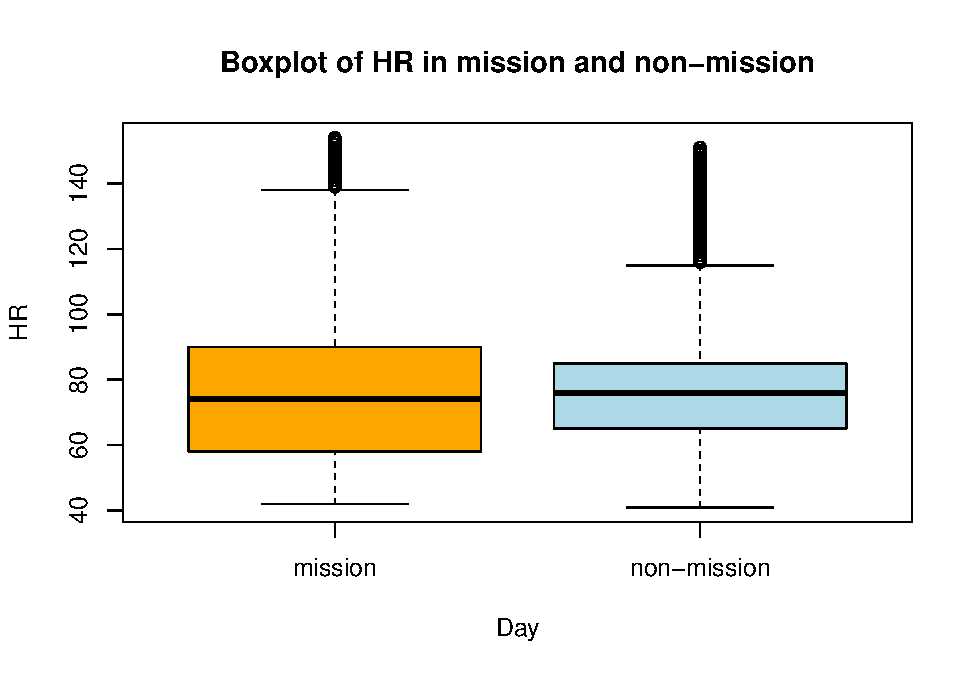
\includegraphics{HW4-Hints_files/figure-latex/unnamed-chunk-14-1.pdf}

\section{Q2 - paired t-test}\label{q2---paired-t-test}

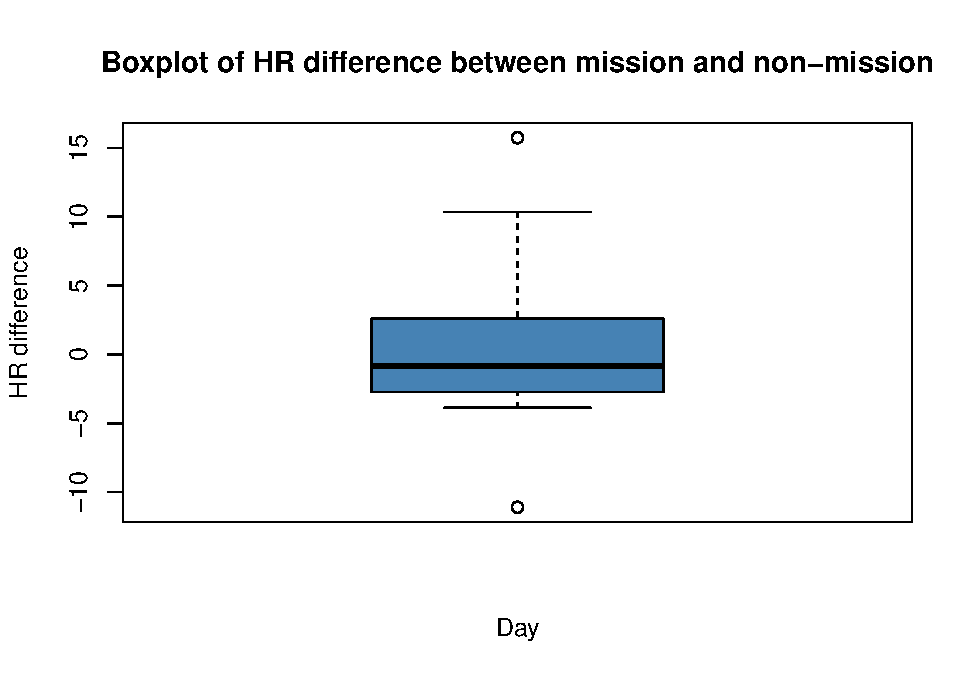
\includegraphics{HW4-Hints_files/figure-latex/unnamed-chunk-16-1.pdf}

\subsection{Q2 - Paired test results}\label{q2---paired-test-results}

\begin{verbatim}
## 
##  Paired t-test
## 
## data:  missions_HR and non_missions_HR
## t = 0.30722, df = 11, p-value = 0.7644
## alternative hypothesis: true mean difference is not equal to 0
## 95 percent confidence interval:
##  -3.767845  4.990359
## sample estimates:
## mean difference 
##       0.6112569
\end{verbatim}

\begin{table}[!h]

\caption{\label{tab:unnamed-chunk-19}Paired t-test}
\centering
\fontsize{8}{10}\selectfont
\begin{tabular}[t]{llrrl}
\toprule
  & Activity & pre\_mis\_p & df & CI\\
\midrule
\cellcolor{gray!6}{df} & \cellcolor{gray!6}{HR} & \cellcolor{gray!6}{0.764} & \cellcolor{gray!6}{11} & \cellcolor{gray!6}{-3.768 - 4.99}\\
\bottomrule
\end{tabular}
\end{table}

\section{Q3 - Plots and Proportion
test}\label{q3---plots-and-proportion-test}

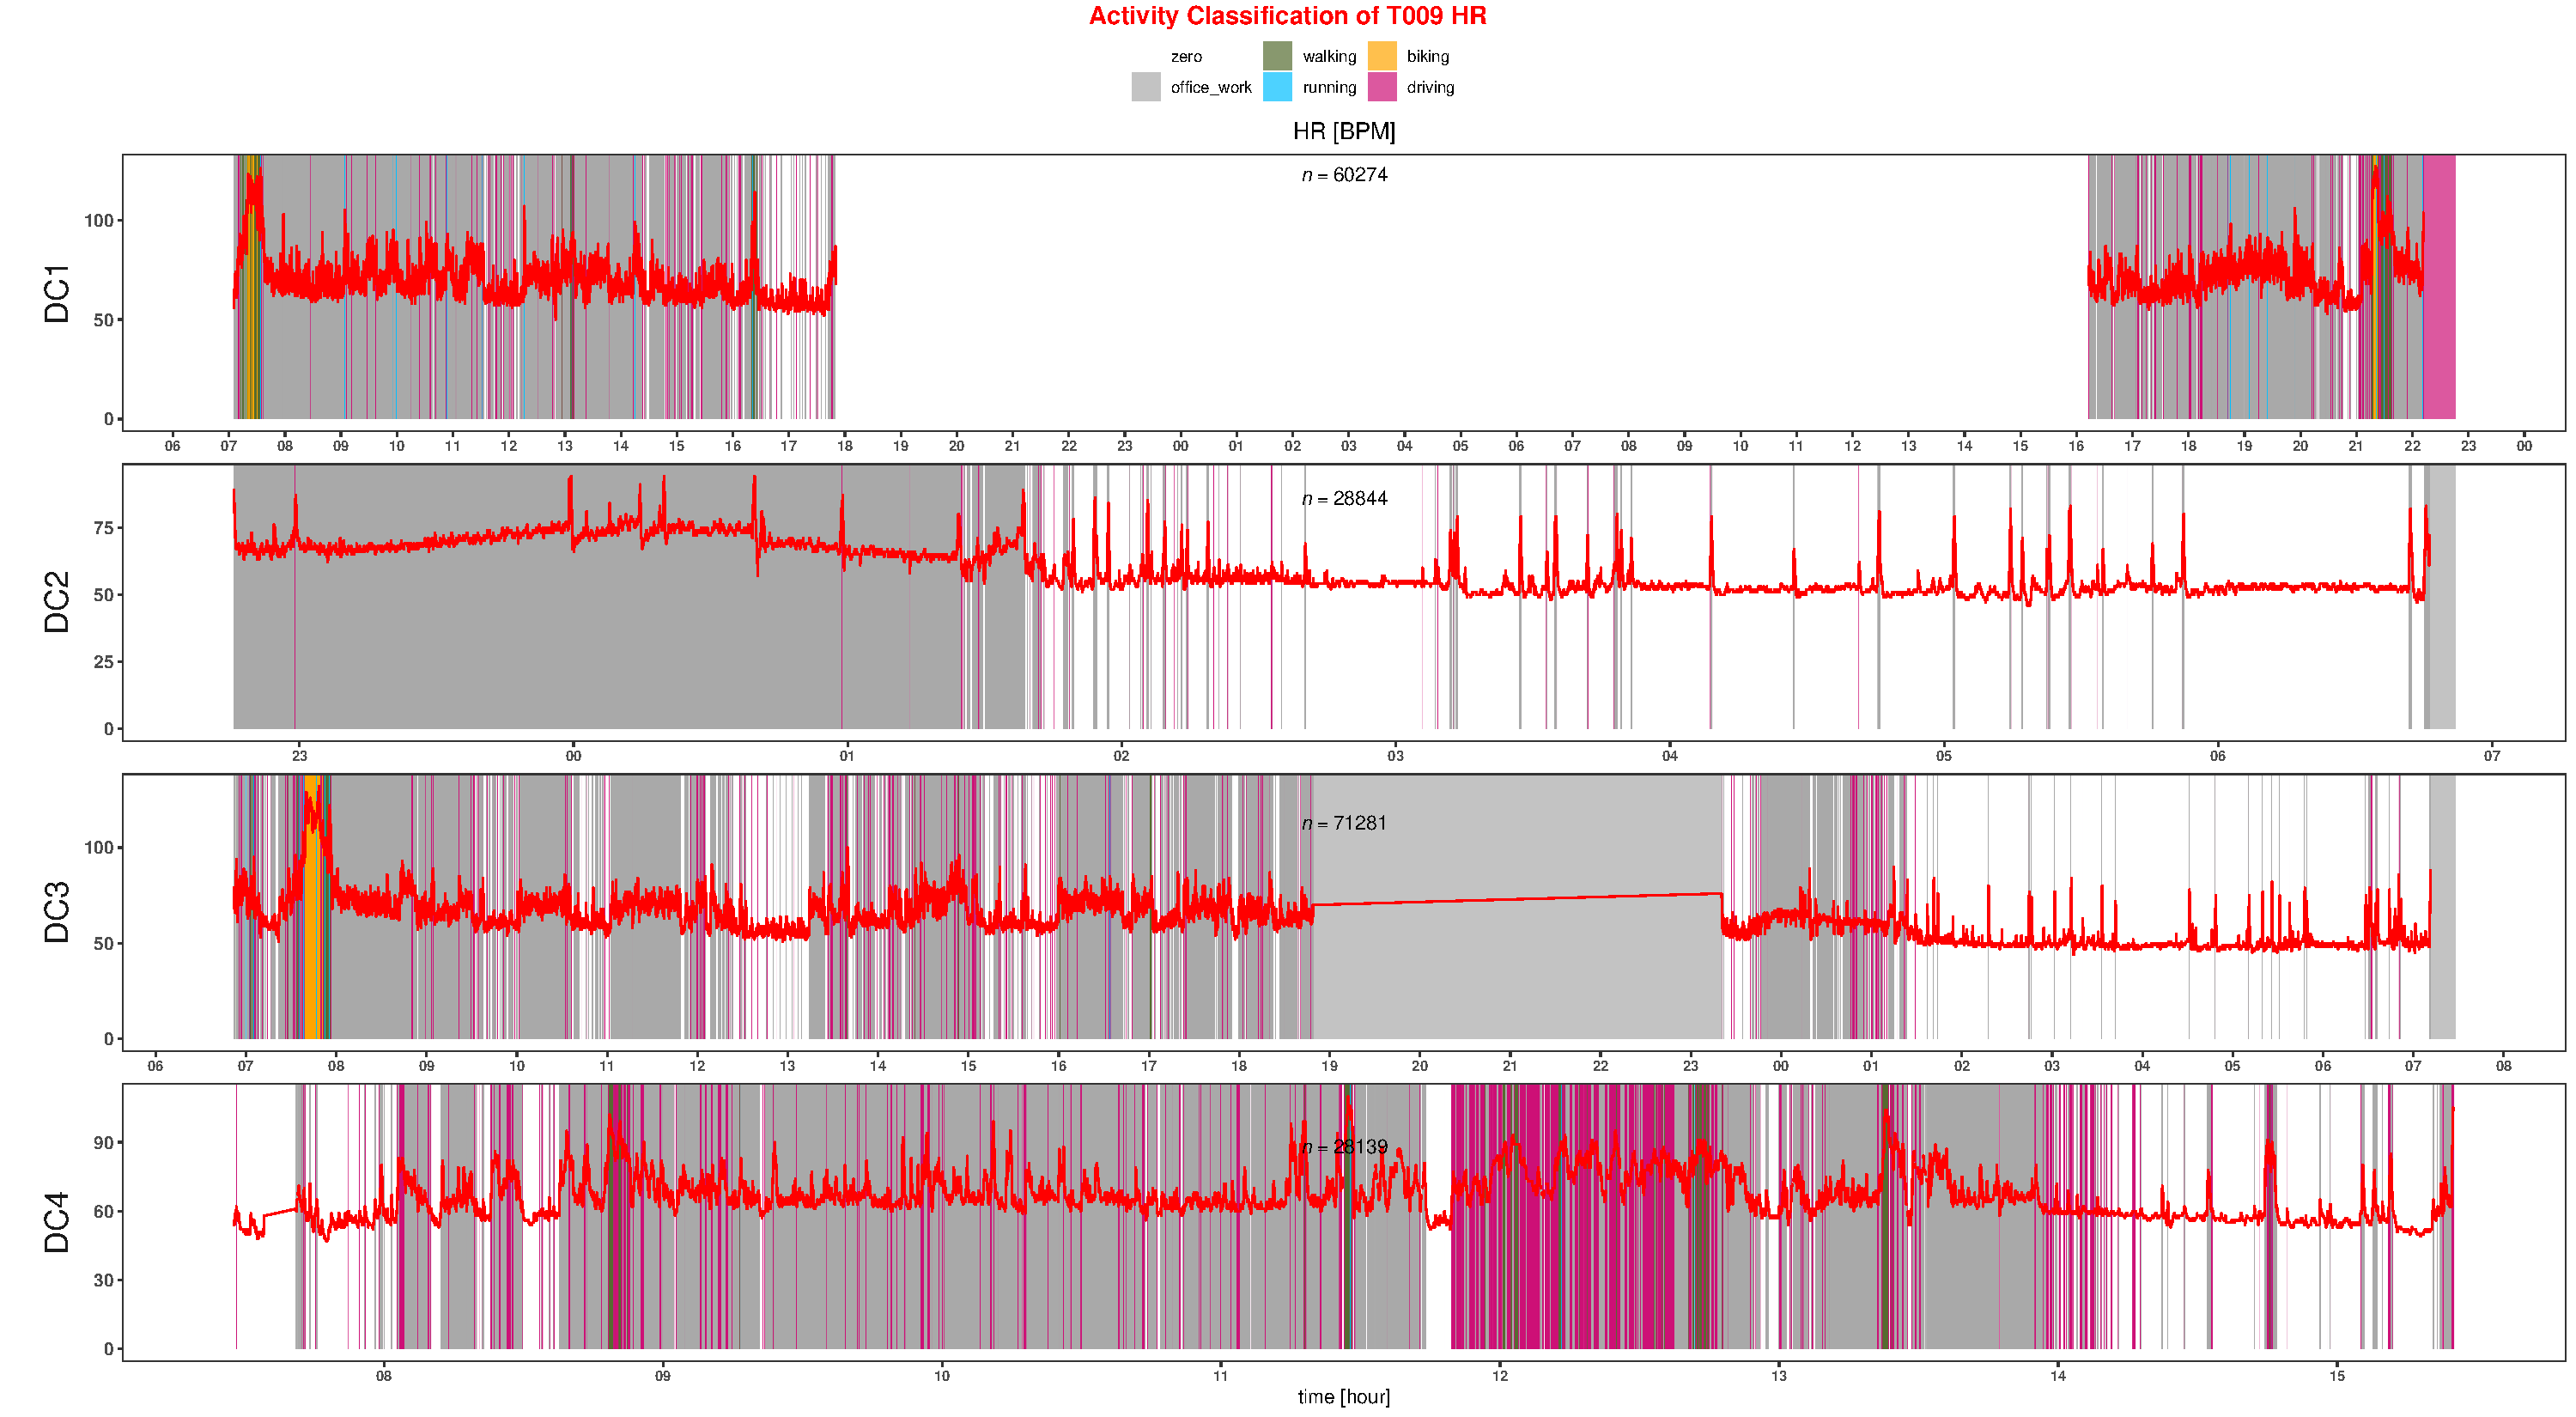
\includegraphics{HW4-Hints_files/figure-latex/unnamed-chunk-20-1.pdf}

\newpage

\section{Q3 - proportion test}\label{q3---proportion-test}

\begin{verbatim}
## `summarise()` has grouped output by 'Day'. You can override using the `.groups`
## argument.
\end{verbatim}

\subsubsection{2-sample test for equality of proportions with continuity
correction}\label{sample-test-for-equality-of-proportions-with-continuity-correction}

\begin{verbatim}
## 
##  2-sample test for equality of proportions with continuity correction
## 
## data:  c(mission_prop * sum(proportion_mission$n), non_mission_prop * sum(proportion_nonMission$n)) out of c(sum(proportion_mission$n), sum(proportion_nonMission$n))
## X-squared = 1659.7, df = 1, p-value < 2.2e-16
## alternative hypothesis: two.sided
## 95 percent confidence interval:
##  0.1365081 0.1434919
## sample estimates:
## prop 1 prop 2 
##   0.98   0.84
\end{verbatim}

\end{document}
